% Section 1.2: information theory and maximum likelihood from first principles.
\section{Cross Entropy, KL Divergence, and Maximum Likelihood}
\label{sec:logreg_to_mlp:cross_entropy_kl_divergence_and_maximum_likelihood}

\begin{keyidea}[Three quantities and three questions]
Entropy asks: how unpredictable is the source itself? Cross-entropy asks: how
surprised will a particular model be by that source? KL divergence asks: how much
extra surprise does using that model create? Maximum likelihood chooses the
model that assigns the greatest joint probability, or density, to the observed
data. These ideas connect through one operation: averaging negative log
probabilities under the distribution that supplies the observations.
\end{keyidea}

\subsection{Start with a robot that must describe what it sees}
A mobile robot sends a stream of corridor events: clear path, person, cart, or
blocked path. Suppose their long-run probabilities are
\[
P=(1/2,1/4,1/8,1/8).
\]
Sending two bits for every event works: there are four possibilities. But the
outcomes are not equally common. Could we give frequent outcomes shorter messages
and rare ones longer messages, reducing the average communication cost?

Now imagine the robot's model predicts a different frequency distribution $Q$.
Even if the communication channel is perfect, a code designed for $Q$ can be
wasteful on events actually drawn from $P$. This is a concrete way to separate
\emph{unavoidable uncertainty} from \emph{avoidable model mismatch}.
The same distinction applies to prediction: a noisy task can have a positive
best possible log loss, while a confident but wrong model adds further loss.

The narrative in this section is
\[
\text{surprise}\longrightarrow\text{average surprise}\longrightarrow
\text{mismatch}\longrightarrow\text{estimating a model from data}.
\]
We first work on a finite outcome space. Continuous measurements need additional
care and are treated explicitly later. Throughout, $P$ is the distribution that
supplies outcomes and $Q$ is the distribution used to score them, unless an
expression explicitly swaps their roles.

\subsection{Why should information be a negative logarithm?}
Suppose an event has probability $p$. We seek a numerical measure $I(p)$ of the
information gained when learning that it occurred. A plausible set of
requirements is:
\begin{enumerate}
\item A certain event gives no new information: $I(1)=0$.
\item A rarer event is more informative: $I(p)$ decreases as $p$ increases.
\item For independent events, information adds: $I(pq)=I(p)+I(q)$.
\item The measure varies continuously with probability.
\end{enumerate}
The independence clause is essential: probabilities multiply for independent
events. For dependent events, the relevant factorization is
$P(A,B)=P(A)P(B\mid A)$, so information adds using a conditional probability.

To see what these requirements imply, set $p=e^{-t}$ and define
$F(t)=I(e^{-t})$ for $t\geq0$. Then
\[
F(t+s)=F(t)+F(s).
\]
For positive integers, repeated addition gives $F(n)=nF(1)$. Dividing an interval
into equal parts gives $F(m/n)=(m/n)F(1)$ for nonnegative rationals. Continuity
extends this to real $t\geq0$. Therefore $F(t)=ct$, with $c>0$ by the rarity
requirement, and
\[
\boxed{I(p)=-c\ln p.}
\]
The choice of $c$ fixes the unit. With base-two logarithms, a fair coin outcome
has information $-\log_2(1/2)=1$ bit. With natural logarithms the unit is a nat.
Since $\log_2 p=\ln p/\ln2$, a value in nats divided by $\ln2$ is its value in
bits. Information here is about reduction of probabilistic uncertainty, not the
semantic importance of a message. A rare sensor glitch can have high surprise
without being useful for navigation.

\paragraph{One event versus a distribution.}
For $P=(1/2,1/4,1/8,1/8)$, the four event surprises are $1,2,3,3$ bits.
A particular observed event has one of these values. Entropy will be the average
of those values before we know which event will occur. Do not confuse the
information of an outcome with the uncertainty of the whole distribution.

\begin{figure}[htbp]
\centering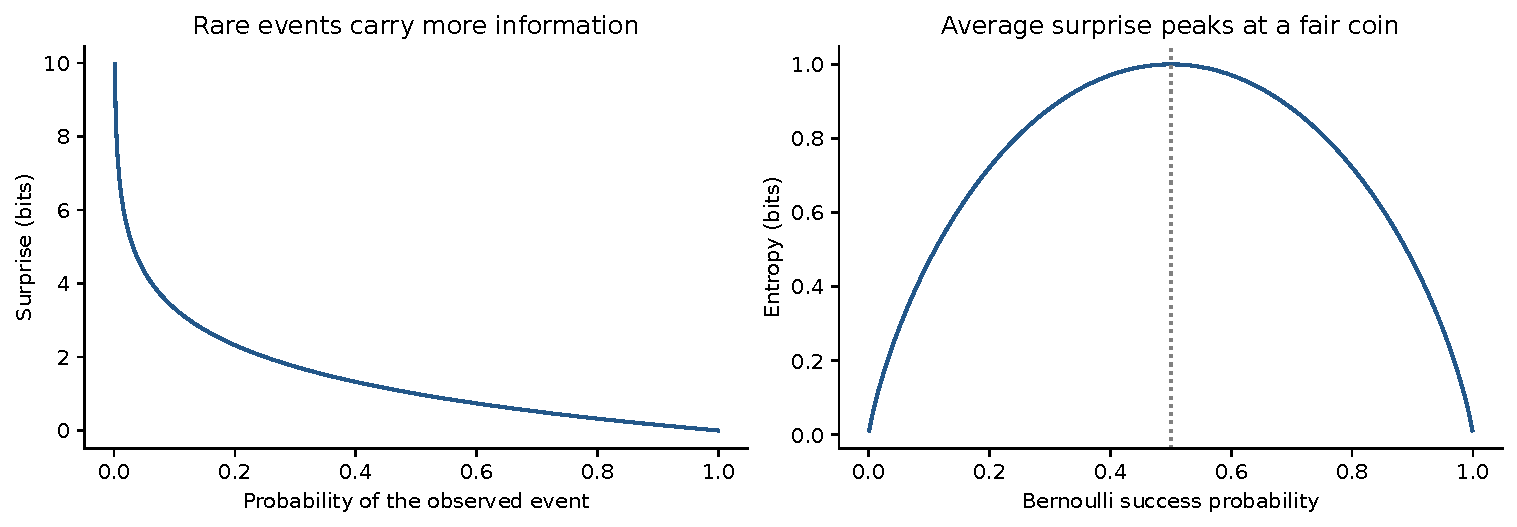
\includegraphics[width=\linewidth]{information_1_2/surprise_entropy.pdf}
\caption{Left: surprise of one event grows as its probability decreases. Right:
the average surprise of a Bernoulli source is largest at equal probabilities.
These curves answer different questions: event surprise and source uncertainty.}
\end{figure}

\subsection{Expectation turns surprise into entropy}
For a finite random variable $X$ with outcomes $x_1,\ldots,x_K$, let
$p_k=P(X=x_k)$. By the definition of expectation, any function $f(X)$ has mean
$\sum_k p_k f(x_k)$. Choosing $f(x)=-\log P(x)$ gives
\begin{equation}
\boxed{H(P)=\mathbb E_{X\sim P}[-\log P(X)]
=-\sum_{k=1}^K p_k\log p_k.}
\label{eq:info12-entropy}
\end{equation}
The weights outside the logarithm describe \emph{how often} an event occurs;
the logarithm describes \emph{how surprising} that event is. Entropy is not
$-\log\mathbb E[P(X)]$, and not an unweighted average over the list of possible
outcomes. Moving a nonlinear logarithm outside an expectation changes the
quantity.

For the robot stream, in bits,
\[
H(P)=\tfrac12(1)+\tfrac14(2)+\tfrac18(3)+\tfrac18(3)=1.75.
\]
This is below the two bits needed by an equiprobable four-outcome source.
A deterministic source has entropy zero: it never surprises an observer who
knows the distribution. On a $K$-outcome space,
\[
0\leq H(P)\leq\log K,
\]
with the upper bound attained by the uniform distribution. We will prove the
upper bound from KL nonnegativity below. Zero-probability events contribute
zero by the continuous extension $\lim_{t\downarrow0}t\log t=0$.

\paragraph{A thought experiment.}
Imagine predicting the next symbol from a fair coin source versus a coin that
comes up heads $99\%$ of the time. For the biased coin, usually there is almost
nothing new to learn, but occasionally a tail is very surprising. Entropy
balances these two facts through a frequency-weighted average. It does not
simply count the number of logically possible outcomes.

\subsection{Coding makes the average operational}
A binary \emph{prefix code} is a collection of bit strings in which no complete
codeword is the prefix of another. This allows concatenated messages to be
decoded without separators. For the robot stream, consider these three codes:
\begin{center}
\begin{tabular}{lrrrr}
\toprule
Event & True $P$ & $P$-matched code & Uniform code & $R$-matched code\\
\midrule
Clear & $1/2$ & 0 & 00 & 110\\
Person & $1/4$ & 10 & 01 & 111\\
Cart & $1/8$ & 110 & 10 & 10\\
Blocked & $1/8$ & 111 & 11 & 0\\
\bottomrule
\end{tabular}
\end{center}
The last code matches $R=(1/8,1/8,1/4,1/2)$. All three are valid prefix codes;
they simply allocate short words differently. Their expected lengths under
$P$ are, respectively,
\[
1.75,\qquad2,\qquad
\tfrac12(3)+\tfrac14(3)+\tfrac18(2)+\tfrac18(1)=2.625\ \text{bits}.
\]
The first code is most efficient for this source. The last makes the common
``clear'' event expensive and saves bits on a rare event instead.

\paragraph{Why ideal lengths are negative log probabilities.}
A complete binary code with lengths $\ell_k$ satisfies
$\sum_k2^{-\ell_k}=1$. Think of each prefix as selecting a fraction
$2^{-\ell_k}$ of the infinite binary tree. Assigning probability $q_k$ the
fraction $q_k$ suggests the ideal length $\ell_k=-\log_2q_k$.
The code tree has only integer depths, however; these ideal lengths need not be
integers. The dyadic probabilities in the table were chosen so they are.

More generally, the Kraft inequality says prefix-code lengths satisfy
$S=\sum_k2^{-\ell_k}\leq1$. Set $r_k=2^{-\ell_k}/S$. Then, in bits,
\[
\mathbb E_P[\ell_X]
=-\sum_kp_k\log_2r_k-\log_2S
=H(P)+D_{\mathrm{KL}}(P\|R)-\log_2S\geq H(P).
\]
This lower bound uses the KL nonnegativity proved shortly. Conversely, choosing
$\ell_k=\lceil-\log_2p_k\rceil$ gives a prefix code with
\[
H(P)\leq\mathbb E_P[\ell_X]<H(P)+1
\]
when the source has positive probabilities on its supported outcomes.
For blocks of $n$ independent events, applying the construction to the block
probabilities gives an overhead of less than one bit \emph{per block}, hence
less than $1/n$ bit per event.

\begin{warning}[Read the slide's coding statement precisely]
Entropy is an ideal average code length and an asymptotically achievable rate
for an i.i.d. source, not necessarily the exact length of a one-symbol binary
code. A Bernoulli source can have entropy $0.2$ bits even though a single
nontrivial binary symbol needs an integer-length codeword. Block coding is how
fractional rates become meaningful. Dependencies require conditional or joint
coding; the marginal entropy alone need not be the best rate for a sequence.
\end{warning}

\subsection{Cross-entropy: keep the source, change the scoring model}
Suppose outcomes still come from $P$, but we evaluate them using probabilities
$q_k=Q(X=x_k)$. The average model-assigned surprise is
\begin{equation}
\boxed{H(P,Q)=\mathbb E_{X\sim P}[-\log Q(X)]
=-\sum_kp_k\log q_k.}
\label{eq:info12-crossentropy}
\end{equation}
The first argument determines the averaging weights. The second determines the
logarithmic score. Swapping the arguments changes both roles. This distinction
is the single most useful way to read a cross-entropy expression.

For the robot source and a uniform model, every event receives two bits of
surprise, so $H(P,Q)=2$. For $R$ above, $H(P,R)=2.625$. In both cases the actual
source remains $P$ and has the same entropy $1.75$.

For a general model $Q$ with positive probability wherever $P$ has positive
probability, the ideal $Q$-based length is $-\log_2q_k$. Rounded Shannon lengths
have expected length between $H(P,Q)$ and $H(P,Q)+1$ bits. This is an ideal or
asymptotic mismatched-coding interpretation; an arbitrary integer code described
as ``optimized for $Q$'' need not have length exactly $-\log_2q_k$.

\paragraph{Support is part of the meaning.}
If $p_k>0$ but $q_k=0$, an event that really can happen has been declared
impossible. Its log loss is infinite, so $H(P,Q)=+\infty$. If $p_k=0$, that
outcome is never scored under $P$ and its term is defined to contribute zero.
Do not evaluate $0\log0$ naively in numerical code.

\begin{figure}[htbp]
\centering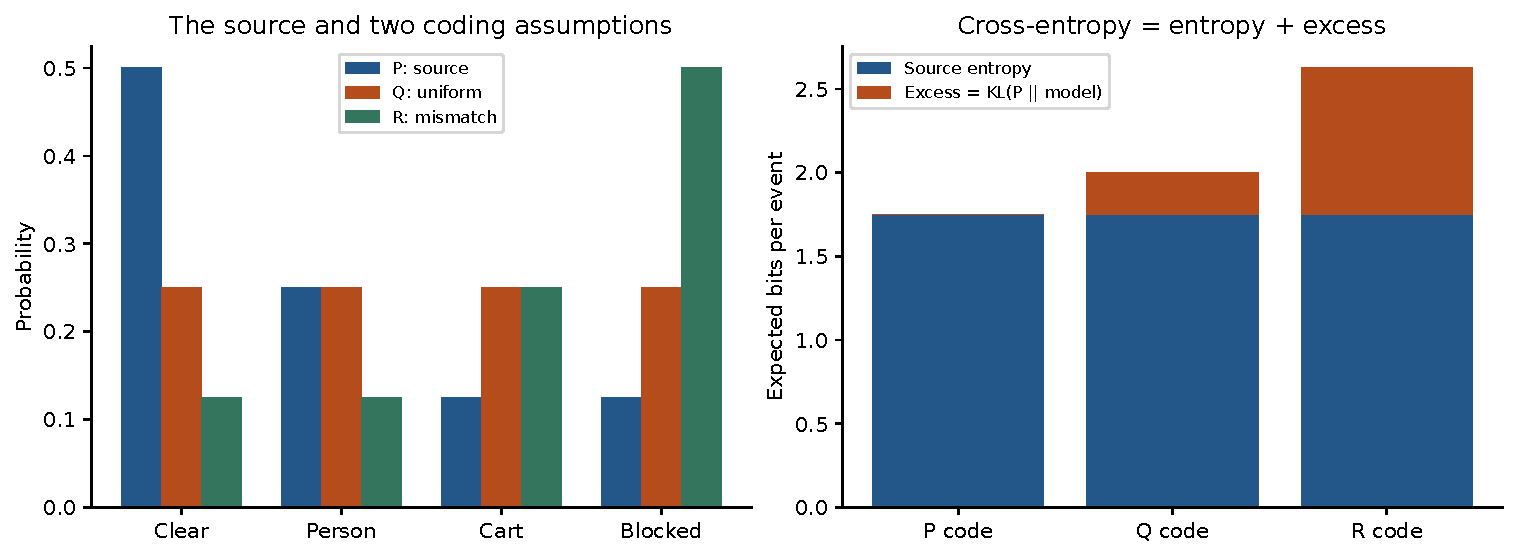
\includegraphics[width=\linewidth]{information_1_2/coding.pdf}
\caption{The same source is scored using three models. The unavoidable source
entropy is unchanged. The additional orange part of each expected code length
is KL divergence. The probabilities are dyadic, so the displayed coding costs
are exact for the prefix codes in the table.}
\end{figure}

\subsection{KL divergence is the excess expected log loss}
Subtract the source entropy from cross-entropy, assuming the expressions are
finite, and collect the logarithms:
\begin{align}
H(P,Q)-H(P)
&=\sum_kp_k\bigl(\log p_k-\log q_k\bigr)\notag\\
&=\sum_kp_k\log\frac{p_k}{q_k}
=\mathbb E_{X\sim P}\!\left[\log\frac{P(X)}{Q(X)}\right]
=:D_{\mathrm{KL}}(P\|Q).
\label{eq:info12-kl}
\end{align}
Equivalently, $D_{\mathrm{KL}}(P\|Q)=-\mathbb E_P\log[Q(X)/P(X)]$,
which matches the slide. Thus
\[
\boxed{H(P,Q)=H(P)+D_{\mathrm{KL}}(P\|Q).}
\]
For infinite quantities, do not treat $+\infty-\infty$ as a legitimate
subtraction; define KL through the log-ratio expression with suitable support
and integrability conditions.

Each individual log ratio may be positive or negative: a model can assign
\emph{more} probability than $P$ to an outcome. KL is the average over $P$.
Normalization forces a tradeoff: giving extra probability to some outcomes
leaves less for others. The average cannot be negative.

\paragraph{Proof of nonnegativity, including zero probabilities.}
The elementary inequality $\log t\leq t-1$ for $t>0$ follows by minimizing
$t-1-\log t$: its derivative is $1-1/t$, and its minimum at $t=1$ is zero.
Let $S=\{k:p_k>0\}$, and first suppose $q_k>0$ on $S$. Applying the inequality
to $t=q_k/p_k$ gives
\begin{align*}
-D_{\mathrm{KL}}(P\|Q)
&=\sum_{k\in S}p_k\log\frac{q_k}{p_k}\\
&\leq\sum_{k\in S}p_k\left(\frac{q_k}{p_k}-1\right)
=\sum_{k\in S}q_k-1\leq0.
\end{align*}
Equality requires $q_k=p_k$ for every $k\in S$ and no probability mass outside
$S$; hence $P=Q$. If $Q$ has a zero on positive $P$ mass, KL is infinite and the
inequality still holds. This proves both nonnegativity and the equality case.

\paragraph{Consequences.}
The best possible predictive distribution under expected log loss is $Q=P$.
Moreover, using the uniform distribution $U_k=1/K$,
\[
D_{\mathrm{KL}}(P\|U)=\sum_kp_k\log p_k+\log K
=\log K-H(P)\geq0,
\]
proving the maximum-entropy bound. An unrestricted distribution family can attain
zero KL; a restricted model family may not contain $P$ and may have a positive
minimum mismatch.

\subsection{Why KL is directed and is not a distance metric}
For a concrete example, use natural logs and
$P=(0.8,0.2)$, $Q=(0.5,0.5)$. Then
\begin{align*}
D_{\mathrm{KL}}(P\|Q)
&=0.8\ln1.6+0.2\ln0.4\approx0.192745,\\
D_{\mathrm{KL}}(Q\|P)
&=0.5\ln0.625+0.5\ln2.5\approx0.223144.
\end{align*}
Different sampling distributions produce different averages. KL is not symmetric
and therefore cannot be a metric; it also does not generally satisfy the
triangle inequality. It is nonnegative and identifies equality, but those two
properties alone do not make a geometric distance.

For an explicit triangle-inequality counterexample, take
$A=(1,0)$, $B=(1/2,1/2)$, and $C=(1/4,3/4)$. Then
$D(A\|C)=\ln4\approx1.3863$, while
$D(A\|B)+D(B\|C)=\ln2+\tfrac12\ln(4/3)\approx0.8370$.
The direct divergence exceeds the sum through the intermediate distribution.

The support asymmetry is even sharper. For $P=(1,0)$ and $Q=(1/2,1/2)$,
$D_{\mathrm{KL}}(P\|Q)=\ln2$, while $D_{\mathrm{KL}}(Q\|P)=+\infty$.
Under $P$ only the first event is sampled. Under $Q$ the second event occurs with
positive probability but is impossible under $P$.

\begin{figure}[htbp]
\centering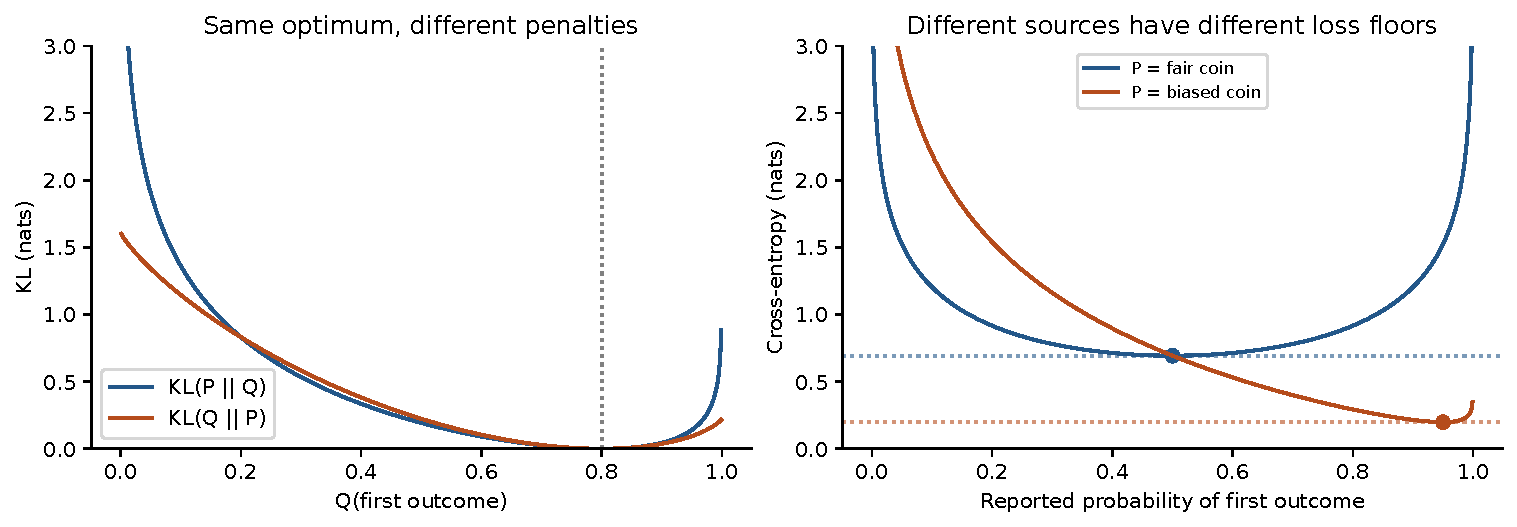
\includegraphics[width=\linewidth]{information_1_2/kl_and_floor.pdf}
\caption{Left: the two directions have the same zero when the distributions
match, but different penalties elsewhere. Right: different true sources have
different minimum cross-entropies. Subtracting each source's entropy isolates
model mismatch. Natural logs are used in both panels.}
\end{figure}

\subsection{Conditioning: knowing the context changes uncertainty}
A robot's observations are not drawn from one label distribution independently
of its inputs. Let $X$ denote the observed context and $Y$ a semantic label.
The relevant uncertainty is the conditional entropy
\[
H_P(Y\mid X)=\mathbb E_{X\sim P_X}
\left[-\sum_y P(y\mid X)\log P(y\mid X)\right].
\]
We average uncertainty \emph{within} each context over how often contexts occur.
Using $P(x,y)=P(x)P(y\mid x)$ and taking negative logs and expectations gives the
chain rule
\[
H_P(X,Y)=H_P(X)+H_P(Y\mid X).
\]
The expected information gained about $Y$ from knowing $X$ is
\[
I_P(X;Y)=H_P(Y)-H_P(Y\mid X)
=D_{\mathrm{KL}}(P_{XY}\|P_XP_Y)\geq0.
\]
This follows by expanding the joint log ratio and collecting the marginal and
conditional terms. Conditioning reduces uncertainty \emph{on average}; a
particular unusual context can have more label entropy than the marginal.

For a conditional model $Q_\theta(y\mid x)$, expected log loss decomposes as
\begin{equation}
\underbrace{\mathbb E_{P_{XY}}[-\log Q_\theta(Y\mid X)]}_{\text{conditional cross-entropy}}
=H_P(Y\mid X)+
\mathbb E_{P_X}D_{\mathrm{KL}}\bigl(P(\cdot\mid X)\|Q_\theta(\cdot\mid X)\bigr).
\label{eq:info12-conditional}
\end{equation}
To derive it, at each fixed $x$ add and subtract
$-\sum_yP(y\mid x)\log P(y\mid x)$, then average over $x$.
This is the version most directly relevant to supervised learning.

\subsection{Maximum likelihood: choosing a model after seeing data}
We now move from two known distributions to an unknown source. Let
$\mathcal D=(x^{(1)},\ldots,x^{(m)})$ be observations drawn independently from a
common but unknown distribution $P_{\mathrm{data}}$. A parametric family
$Q_\theta$ is a set of candidate distributions indexed by $\theta$.

Before observing data, $Q_\theta(x)$ is a probability as a function of $x$ for a
fixed parameter. After observing the data, the same formula, considered as a
function of $\theta$, is a \emph{likelihood}. The data are held fixed while we
compare models:
\[
\mathcal L(\theta;\mathcal D)
=Q_\theta(\mathcal D),\qquad
\hat\theta_{\mathrm{ML}}\in\argmax_\theta\mathcal L(\theta;\mathcal D).
\]
We use membership in the argmax set because a maximizer might not be unique.
There can also be no finite maximizer, as with separable unregularized logistic
regression in Section 1.1. An \emph{estimator} is a rule mapping a dataset to a
parameter value; before sampling, it is itself random. Its realized output is
an estimate.

Likelihood is not a posterior probability of $\theta$. A posterior requires a
prior through Bayes' rule. A high likelihood also does not by itself establish
that the family is correct, or that the estimate will generalize.

\paragraph{Why independence appears in the derivation.}
Under the i.i.d. assumption,
\[
Q_\theta(\mathcal D)=\prod_{i=1}^m Q_\theta(x^{(i)}).
\]
For correlated observations, one instead needs an appropriate joint model, for
example
\[
Q_\theta(x^{(1)})\prod_{i=2}^mQ_\theta(x^{(i)}\mid x^{(1:i-1)}).
\]
The logarithm still turns a product into a sum, but the factors are conditional.
Treating adjacent robot-video frames as independent is a modeling assumption,
not an automatic consequence of having stored them in separate rows.

\subsection{The empirical distribution: turning a dataset into an expectation}
For discrete outcomes, define
\[
\hat P_m(x)=\frac1m\sum_{i=1}^m\mathbf 1\{x^{(i)}=x\}.
\]
It is the observed relative frequency of each outcome. Repeated observations
count repeatedly. For any function $f$,
\begin{align*}
\mathbb E_{\hat P_m}[f(X)]
&=\sum_x\left[\frac1m\sum_i\mathbf1\{x^{(i)}=x\}\right]f(x)\\
&=\frac1m\sum_i\sum_x\mathbf1\{x^{(i)}=x\}f(x)
=\frac1m\sum_i f(x^{(i)}).
\end{align*}
This is why a sample average can be written as an expectation: we have changed
the averaging distribution to the empirical one. It is not an assertion that
$\hat P_m$ equals the unknown true distribution.

For the sequence $(A,A,A,B,C)$, the empirical distribution over $(A,B,C)$ is
$(3/5,1/5,1/5)$, not $(1/3,1/3,1/3)$. If we instead regard the five observation
\emph{indices} as equally likely, each has mass $1/5$; mapping indices to their
values combines the repeated $A$ outcomes. Keeping those spaces distinct avoids
many empirical-entropy mistakes.

\subsection{Every step of the MLE--cross-entropy--KL equivalence}
For a discrete i.i.d. model with probabilities positive on observed outcomes,
\begin{align}
\argmax_\theta Q_\theta(\mathcal D)
&=\argmax_\theta\prod_{i=1}^m Q_\theta(x^{(i)})
&&\text{(independence)}\notag\\
&=\argmax_\theta\sum_{i=1}^m\log Q_\theta(x^{(i)})
&&\text{(monotone log)}\notag\\
&=\argmax_\theta\frac1m\sum_{i=1}^m\log Q_\theta(x^{(i)})
&&\text{(positive scaling)}\notag\\
&=\argmax_\theta\mathbb E_{\hat P_m}\log Q_\theta(X)
&&\text{(empirical mean)}\notag\\
&=\argmin_\theta\mathbb E_{\hat P_m}[-\log Q_\theta(X)]
&&\text{(negation)}\notag\\
&=\argmin_\theta H(\hat P_m,Q_\theta)
&&\text{(definition)}\notag\\
&=\argmin_\theta\{H(\hat P_m,Q_\theta)-H(\hat P_m)\}
&&\text{(constant in $\theta$)}\notag\\
&=\argmin_\theta D_{\mathrm{KL}}(\hat P_m\|Q_\theta).
\label{eq:info12-mlechain}
\end{align}
These are equal sets of optimizers, not equal numerical objectives.
In particular, the sum of log probabilities equals $m$ times the empirical
expectation, not the expectation itself. The factor disappears only because a
positive constant does not change the argmax. Likewise, removing empirical
entropy changes the objective value but not its optimizer or gradient.

\paragraph{Which way does the KL point?}
The empirical distribution comes first: it supplies the data being averaged.
The model comes second: its probabilities are evaluated on those data.
This is forward KL, $D_{\mathrm{KL}}(\hat P_m\|Q_\theta)$, not
$D_{\mathrm{KL}}(Q_\theta\|\hat P_m)$. The order is determined by the likelihood
calculation, not by a freely chosen convention.

\paragraph{Population interpretation.}
If the relevant expectations are finite, the population objective is
\[
\mathbb E_{P_{\mathrm{data}}}[-\log Q_\theta(X)]
=H(P_{\mathrm{data}})+D_{\mathrm{KL}}(P_{\mathrm{data}}\|Q_\theta).
\]
Training substitutes a sample average for this unknown expectation. A law of
large numbers gives convergence for a fixed $\theta$ under suitable assumptions;
consistency of the \emph{optimizer} requires additional conditions, such as
identifiability and control of the objective over the family. Finite-sample
maximum likelihood does not automatically find the true distribution.
If the family is misspecified, even a population-optimal parameter can retain
positive KL.

\subsection{Worked MLEs: Bernoulli and categorical models}
For a Bernoulli model $Q_\theta(1)=\theta$, let $s$ of $m$ labels be one. The
likelihood of the observed ordered sequence is
\[
\mathcal L(\theta)=\theta^s(1-\theta)^{m-s}.
\]
If only the count is observed, its binomial probability includes
$\binom ms$, but this factor is independent of $\theta$ and leaves the estimate
unchanged. For $0<s<m$,
\[
\frac{d}{d\theta}\log\mathcal L(\theta)
=\frac{s}{\theta}-\frac{m-s}{1-\theta}=0
\quad\Longrightarrow\quad\hat\theta=\frac{s}{m}.
\]
The second derivative is $-s/\theta^2-(m-s)/(1-\theta)^2<0$, proving this is the
unique interior maximum. Seven successes in ten trials therefore give $0.7$.
With all successes the maximum is at $\theta=1$ if the closed interval $[0,1]$
is allowed; a finite-logit parameterization cannot reach it and only approaches
the supremum. Parameter space matters.

\begin{figure}[htbp]
\centering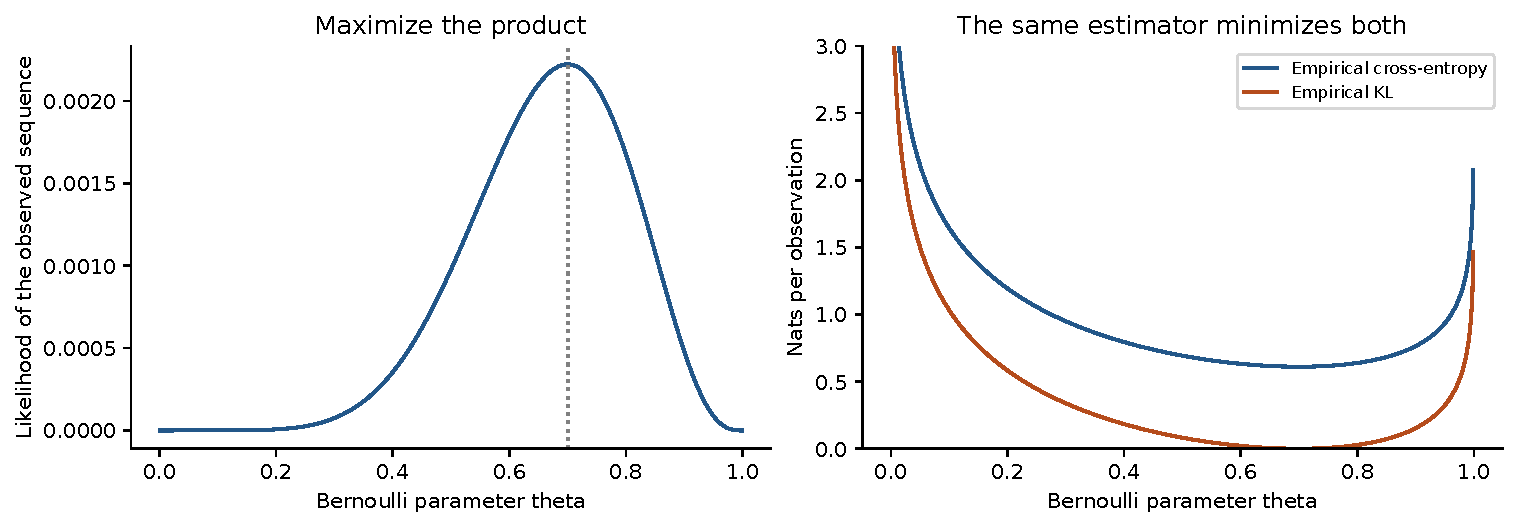
\includegraphics[width=\linewidth]{information_1_2/mle.pdf}
\caption{Seven successes and three failures. The product likelihood peaks at
$0.7$. Mean negative log-likelihood and empirical KL have the same minimizer;
their vertical separation is the entropy of the empirical Bernoulli distribution.}
\end{figure}

For a $K$-class categorical model with counts $n_k$ and probabilities $q_k$,
maximize $\sum_kn_k\log q_k$ subject to $\sum_kq_k=1$.
When all counts are positive, the Lagrangian
\[
\Lambda(q,\lambda)=\sum_kn_k\log q_k+\lambda\left(1-\sum_kq_k\right)
\]
gives $n_k/q_k=\lambda$. Summing $q_k=n_k/\lambda$ gives $\lambda=m$, so
$q_k=n_k/m$. Concavity of the log objective makes this a global optimum.
Zero-count classes obtain zero probability in the unrestricted closed simplex;
this can produce infinite future log loss if a previously unseen class appears.
Pseudocounts or priors can address that issue, but then the estimator is no
longer this unregularized maximum-likelihood estimator. With a finite softmax
parameterization, zero probabilities are approached only as limits.

\subsection{Continuous data: densities are not point probabilities}
A continuous measurement such as position has $P(X=x)=0$ at every individual
point, so a continuous-data likelihood uses a \emph{density} $q_\theta(x)$, not
point mass. For a small measurement bin of width $\Delta$,
\[
P_\theta(x\leq X<x+\Delta)\approx q_\theta(x)\Delta.
\]
With a fixed measurement scale, the product of $\Delta$ factors does not depend
on $\theta$, explaining why maximizing the density likelihood is meaningful.
A density can exceed one, and a negative log density can be negative.

For densities $p,q$ relative to the same base measure, define differential
entropy and cross-entropy when the integrals exist:
\[
h(P)=-\int p(x)\log p(x)\,dx,\qquad
h(P,Q)=-\int p(x)\log q(x)\,dx.
\]
Unlike discrete entropy, differential entropy can be negative and depends on
units. For $U=aX+b$, $a\ne0$, change of variables yields
\[
p_U(u)=\frac{p_X((u-b)/a)}{|a|},\qquad
h(U)=h(X)+\log|a|.
\]
Converting meters to centimeters adds $\log100$ nats. Differential entropy by
itself is therefore not an absolute number of bits needed to encode a real
number exactly. Fine quantization gives, under appropriate regularity,
$H(X_\Delta)\approx h(X)+\log(1/\Delta)$ in one dimension.

By contrast,
\[
D_{\mathrm{KL}}(P\|Q)=\int p(x)\log\frac{p(x)}{q(x)}\,dx
\]
is invariant under a common invertible smooth coordinate transformation: the
Jacobian factors cancel inside the density ratio, and the outer measure changes
consistently. It remains nonnegative, and it equals $h(P,Q)-h(P)$ when that
subtraction is well defined.

\begin{warning}[A subtle limit of the empirical-KL shorthand]
For continuous observations, the empirical measure is
$\hat P_m=m^{-1}\sum_i\delta_{x^{(i)}}$, a collection of point masses.
A smooth density model assigns zero probability to that finite set, whereas
$\hat P_m$ assigns it probability one. Thus
$D_{\mathrm{KL}}(\hat P_m\|Q_\theta)=+\infty$ in the literal measure-theoretic
sense. The finite sample negative log-density is still a valid MLE objective,
but it is not a finite KL between those two measures. Use the population-density
KL interpretation, or explicitly discretize/smooth consistently. The discrete
chain in \eqref{eq:info12-mlechain} should not be transferred blindly to Dirac
empirical measures and continuous densities.
\end{warning}

This issue does not invalidate conditional classification: for each observed
input, the predicted distribution over a finite set of labels is discrete.
The per-example categorical cross-entropy remains well defined even when the
input itself is continuous.

\subsection{Interpreting the slide: approximating two modes by one Gaussian}
Suppose a robot's position belief has two plausible locations because two
corridors look similar. Use the explicit illustrative density
\[
p(x)=\tfrac12\mathcal N(x;-3,0.7^2)+\tfrac12\mathcal N(x;3,0.7^2).
\]
We are forced to summarize it with a single Gaussian
$q_{\mu,s}(x)=\mathcal N(x;\mu,s^2)$, $s>0$. No member of this family can
represent both narrow peaks faithfully. Which compromise does each KL choose?

\paragraph{Forward KL: derive the moment-matching solution.}
Minimizing $D_{\mathrm{KL}}(P\|Q_{\mu,s})$ is equivalent to minimizing
$\mathbb E_P[-\log q_{\mu,s}(X)]$, because $h(P)$ is constant. The Gaussian
negative log density gives
\[
h(P,Q_{\mu,s})=\frac12\log(2\pi s^2)
+\frac{\mathbb E_P[(X-\mu)^2]}{2s^2}.
\]
Let $m_P=\mathbb E_P X$ and $v_P=\operatorname{Var}_P X$. Expanding
$X-\mu=(X-m_P)+(m_P-\mu)$ and noting the cross term has mean zero gives
\[
\mathbb E_P[(X-\mu)^2]=v_P+(m_P-\mu)^2.
\]
For any $s$, the minimizing mean is $\mu=m_P$. Write $v=s^2$; then
\[
\frac{d}{dv}\left[\frac12\log(2\pi v)+\frac{v_P}{2v}\right]
=\frac{v-v_P}{2v^2}.
\]
It is negative below $v_P$ and positive above, so the minimizing variance is
$v=v_P$ when $v_P>0$. For our symmetric mixture,
\[
\boxed{\mu^*=0,\qquad(s^*)^2=3^2+0.7^2=9.49,
\qquad s^*\approx3.0806.}
\]
The broad fitted Gaussian covers both modes, even though it assigns appreciable
density to the low-probability region between them. Ignoring either mode would
make many $P$-drawn observations extremely surprising. That is what forward KL
penalizes. The mean position zero is a statistical summary, not necessarily a
physically plausible robot location.

\paragraph{Reverse KL: why a single mode can win.}
The reverse objective is
\[
D_{\mathrm{KL}}(Q_{\mu,s}\|P)
=\mathbb E_Q[\log q_{\mu,s}(X)-\log p(X)]
=-h(Q_{\mu,s})-\mathbb E_Q\log p(X).
\]
Now the fitted model supplies the samples. A broad $Q$ generates many samples
between the two peaks, where $p(x)$ is tiny, producing a large penalty. A narrow
$Q$ centered near one peak rarely visits the valley or the other peak. Missing
the other mode is less directly penalized because expectations are under $Q$.
The $-h(Q)$ term matters too: it discourages collapsing a continuous Gaussian
to an infinitesimally narrow spike. Reverse KL is not merely ``maximize $p$ at
the model mean.''

Near the left mode, if the peaks are well separated,
$p(x)\approx\tfrac12\mathcal N(x;-3,0.7^2)$. Choosing $Q$ close to that component
makes $\log(q/p)\approx\log2$, so its reverse KL is roughly $0.6931$ nats.
The companion script searches Gaussian mean and scale on a grid, refines the
best grid neighborhood, and evaluates expectations by Gauss--Hermite quadrature.
It finds a fit near $(\mu,s)=(-3,0.7)$ with reverse KL about $0.69312$.
By symmetry a corresponding fit near $(3,0.7)$ has the same value. This numerical
search supports the displayed example; it is not a theorem that reverse KL
always selects exactly one mode or a proof of global optimality for every
mixture.

\begin{figure}[htbp]
\centering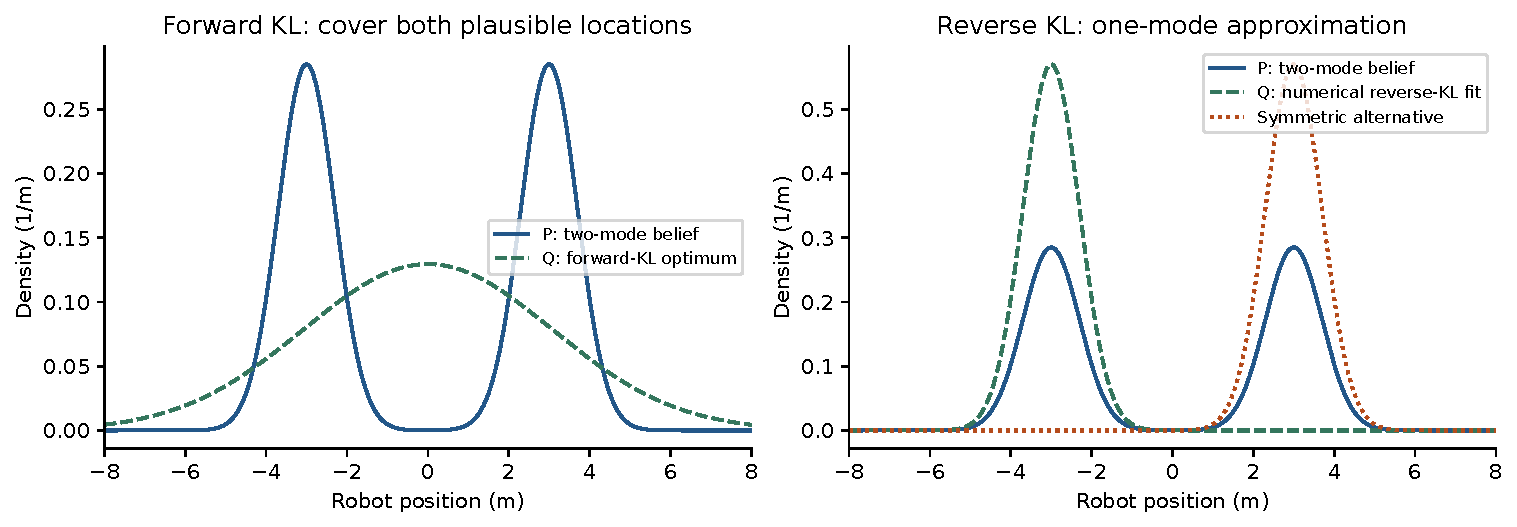
\includegraphics[width=\linewidth]{information_1_2/mixture_direction.pdf}
\caption{A constructed counterpart of the slide's qualitative example, with
explicit distributions. Forward KL has an analytically derived Gaussian optimum.
Reverse KL has two symmetric one-mode candidates found numerically. The mismatch
is unavoidable because a single Gaussian cannot express this two-mode belief.}
\end{figure}

\begin{figure}[htbp]
\centering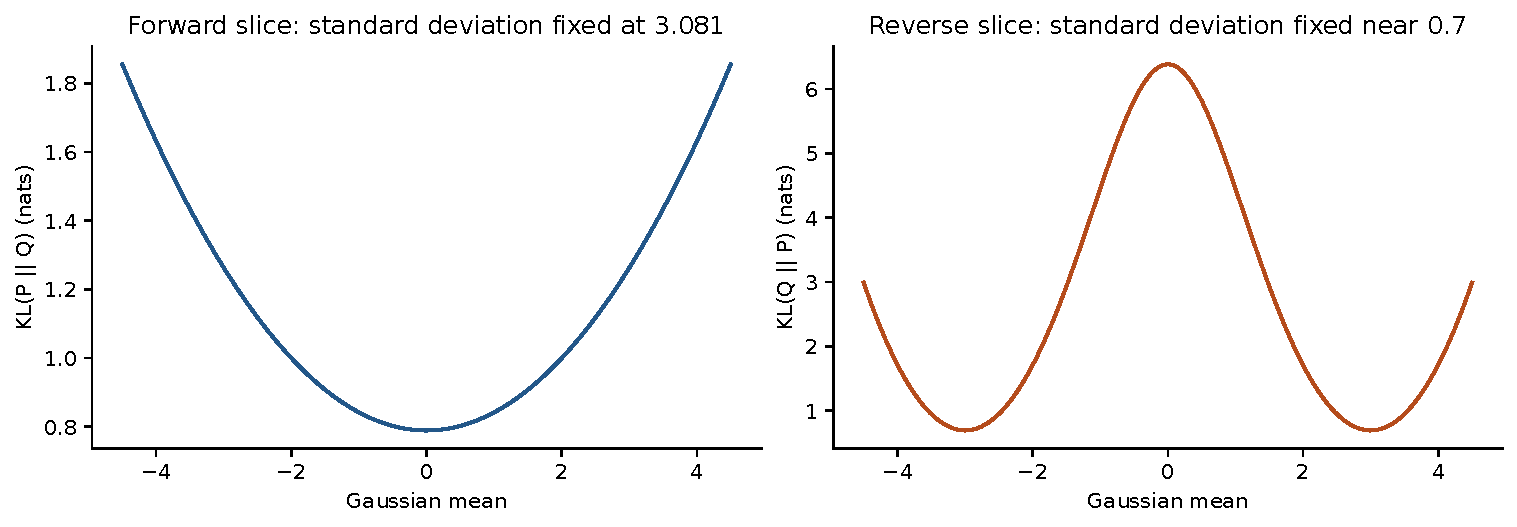
\includegraphics[width=\linewidth]{information_1_2/mixture_objectives.pdf}
\caption{One-dimensional slices through two different objectives. Each panel
holds the standard deviation at its displayed fitted value and varies the mean.
The forward slice favors the midpoint; the reverse slice favors either peak.
These slices are not the full two-parameter optimization landscapes.}
\end{figure}

\paragraph{When the slogan fails.}
``Forward KL covers modes; reverse KL seeks modes'' is a useful tendency for
restricted approximating families and well-separated targets. If the family
contains $P$, both directions can achieve the exact match. Overlapping modes,
unequal mixture weights, or a richer family can change the compromise. Neither
direction is universally better. For localization, throwing away a plausible
mode can hide ambiguity, while a broad Gaussian can place probability in
impossible corridors. A multimodal representation may be preferable to either
single-Gaussian approximation.

\paragraph{Why maximum likelihood is the left-hand case.}
MLE averages $-\log q_\theta(x)$ over \emph{observed data}. It asks whether the
model makes the data plausible, giving forward KL in the population/discrete
interpretation. It does not sample from $Q_\theta$ and ask whether those samples
are plausible under $P$. Reverse-KL objectives arise in other settings, but do
not follow from the likelihood derivation just given.

\subsection{Transfer question 1: why track KL rather than cross-entropy?}
Because KL removes the uncertainty floor. A perfect model of a fair binary
source still has cross-entropy $\log2\approx0.6931$ nats. A perfect model of a
source with probabilities $(0.95,0.05)$ has cross-entropy about $0.1985$ nats.
Both have KL zero. A larger cross-entropy does not necessarily mean the model is
further from its source; the source may simply be less predictable.

For a fixed known $P$, KL states the excess expected loss relative to the
unrestricted optimum $Q=P$. For example, if $H(P)=0.60$ and $H(P,Q)=0.65$,
the model pays $0.05$ extra nats per observation. Cross-entropy alone would not
reveal that gap unless we knew the entropy floor.

\paragraph{Three qualifications make this useful in practice.}
First, with $P$ fixed, subtracting $H(P)$ leaves gradients and optimizer locations
unchanged. Computing KL does not improve optimization by itself. Second, if the
model family cannot represent $P$, its best attainable KL may be positive.
The actual optimization gap within that family is
\[
D_{\mathrm{KL}}(P\|Q_\theta)-\inf_{\vartheta}
D_{\mathrm{KL}}(P\|Q_\vartheta),
\]
not simply $D_{\mathrm{KL}}(P\|Q_\theta)$. Third, true $P$ and its entropy are
usually unknown. Held-out samples let us estimate cross-entropy, while estimating
entropy accurately can be difficult, especially in high dimensions.

If labels are represented by one-hot targets, the target entropy for each
example is zero, so per-example cross-entropy and KL to that point mass are
numerically the same. That does not prove the true conditional label entropy is
zero. With noisy or ambiguous labels, the real uncertainty can remain positive.
Known simulator distributions, repeated outcomes at the same finite context,
or soft target distributions are settings in which the entropy subtraction can
be directly informative.

\subsection{Transfer question 2: derive binary cross-entropy as a special case}
For an input $x_n$, the model's distribution over labels $0,1$ is
\[
Q_n=(1-\hat y_n,\hat y_n),\qquad
\hat y_n=p_w(Y=1\mid x_n).
\]
The observed label $y_n\in\{0,1\}$ defines a target distribution concentrated on
that outcome:
\[
P_n=(1-y_n,y_n).
\]
Substituting these two probability vectors into the general finite-outcome
cross-entropy, with the sum over \emph{labels}, gives
\begin{align*}
H(P_n,Q_n)
&=-\sum_{k\in\{0,1\}}P_n(k)\log Q_n(k)\\
&=-(1-y_n)\log(1-\hat y_n)-y_n\log\hat y_n.
\end{align*}
Averaging over the $N$ observations gives exactly the lecture formula:
\[
\boxed{L(w)=-\frac1N\sum_{n=1}^N
\left[y_n\log\hat y_n+(1-y_n)\log(1-\hat y_n)\right].}
\]
There are two different averages: the inner sum is over possible labels at a
fixed input; the outer sum is over dataset examples. The labels and predictions
across all examples are not themselves one normalized probability vector.

An equivalent joint construction avoids ambiguity: put mass $1/N$ on each
example index $n$, and define
$P(n,k)=N^{-1}\mathbf1\{k=y_n\}$ and
$Q_w(n,k)=N^{-1}Q_n(k)$. Then
\[
H(P)=\log N,\quad H(P,Q_w)=\log N+L(w),\quad
D_{\mathrm{KL}}(P\|Q_w)=L(w).
\]
This index-based joint space is not the same as grouping repeated inputs into
an empirical conditional label distribution, whose entropy may be positive.
Both constructions produce the same averaged conditional log loss; they assign
entropy to different random variables.

\paragraph{Soft targets and more than two classes.}
If a target supplies a probability $r_n\in[0,1]$ rather than a hard label,
replace $y_n$ by $r_n$. The same formula becomes the cross-entropy between two
Bernoulli distributions. Its KL equals that BCE minus the target entropy.
For $K$ classes, target probabilities $r_{nk}$ and predictions $q_{nk}$ give
\[
L=-\frac1N\sum_n\sum_{k=1}^K r_{nk}\log q_{nk}.
\]
With one-hot targets this reduces to the negative log probability of the correct
class. Label smoothing changes the target distribution, hence also its entropy
and the optimum; it is not merely a different algebraic form of the original
hard-label objective.

\subsection{Worked semantic-perception example: separate uncertainty from error}
Consider a robot semantic classifier with labels free space, person, and cart.
For a transparent teaching example, the input has only two discrete contexts:
open floor and occluded view. In 100 observations of each context, the label
counts are
\begin{center}
\begin{tabular}{lrrr}
\toprule
Context & Free & Person & Cart\\
\midrule
Open floor & 80 & 15 & 5\\
Occluded view & 10 & 20 & 70\\
\bottomrule
\end{tabular}
\end{center}
The empirical conditional distributions are
$\hat P_A=(0.80,0.15,0.05)$ and $\hat P_B=(0.10,0.20,0.70)$.
Suppose a model predicts
$Q_A=(0.70,0.20,0.10)$ and $Q_B=(0.20,0.30,0.50)$.
Both contexts have weight $1/2$ in this dataset. Directly from the counts,
\[
\mathrm{NLL}_{\mathrm{mean}}
=-\frac1{200}\sum_{c\in\{A,B\}}\sum_k n_{ck}\log Q_c(k)
\approx0.764413\ \text{nats}.
\]
The empirical conditional entropy and mismatch are
\begin{align*}
\hat H(Y\mid X)&=\tfrac12H(\hat P_A)+\tfrac12H(\hat P_B)
\approx0.707344,\\
\hat D&=\tfrac12D_{\mathrm{KL}}(\hat P_A\|Q_A)
+\tfrac12D_{\mathrm{KL}}(\hat P_B\|Q_B)
\approx0.057069.
\end{align*}
They add to $0.764413$, as predicted by \eqref{eq:info12-conditional}.
An unrestricted categorical model per context would fit the empirical frequencies
and reduce the empirical KL to zero, but its cross-entropy would remain
$0.707344$. The remaining label variation cannot be predicted from these two
context categories in this empirical model.

\begin{figure}[htbp]
\centering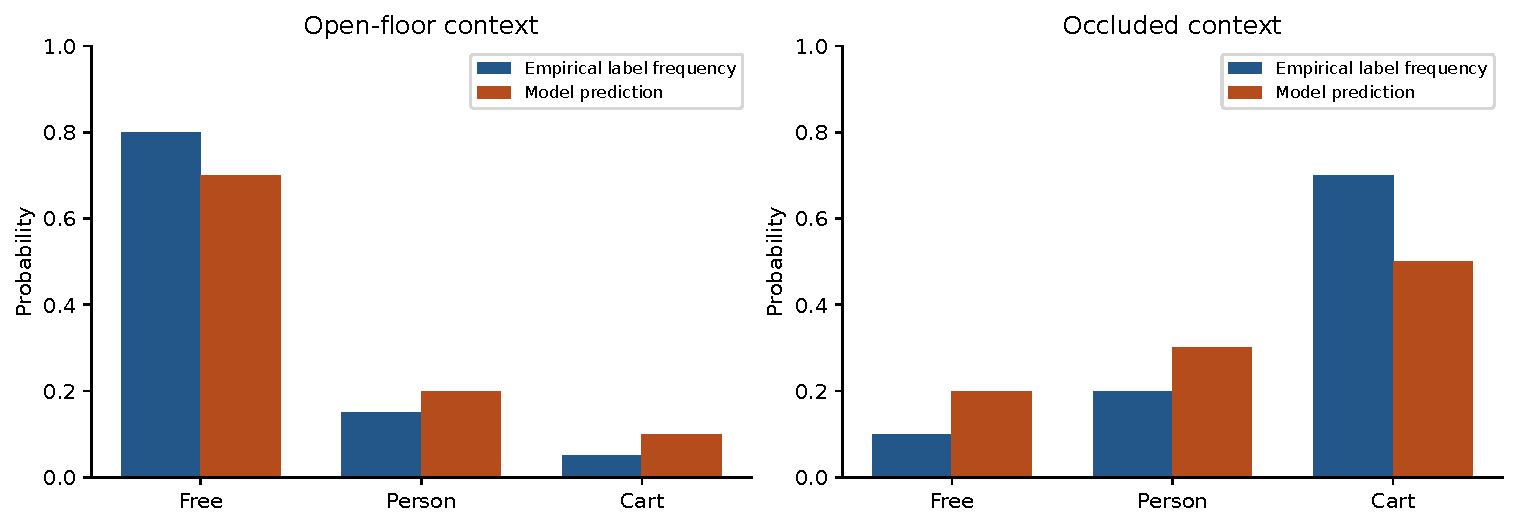
\includegraphics[width=\linewidth]{information_1_2/conditional_robot.pdf}
\caption{The robot example's target frequencies and model probabilities.
The occluded context underpredicts carts; the resulting conditional KL measures
that mismatch separately from the label variability within each context.}
\end{figure}

This is an in-sample decomposition of constructed counts, not an estimate of
irreducible uncertainty on all future robot observations. Richer inputs might
resolve ambiguity; finite frequencies are noisy; context proportions can shift.
For a real study, fit models on training data, compare predictive log loss on
held-out objects or sessions, and report how any entropy estimate was obtained.
Do not estimate an entropy floor from the same overfit model and then call it
known ground truth.

\subsection{Implement the definitions without hiding their edge cases}
The companion uses NumPy for the definitions and numerical experiments.
A stable finite-distribution KL calculation must ignore zero $P$ terms while
returning infinity when positive $P$ meets zero $Q$:
\begin{lstlisting}
def kl(p, q):
    p = np.asarray(p, dtype=float)
    q = np.asarray(q, dtype=float)
    # Validate matching shapes, nonnegativity and sums of one first.
    active = p > 0
    if np.any(q[active] == 0):
        return float("inf")
    return np.sum(p[active] *
                  (np.log(p[active]) - np.log(q[active])))
\end{lstlisting}
The full script validates probability vectors and supports bits or nats.
Using a mask before evaluating logarithms avoids invalid inactive terms.
Adding an arbitrary epsilon to every probability changes the distributions and
may destroy normalization. If smoothing is intended, define and normalize the
smoothed model explicitly. For network outputs, compute log probabilities from
logits using stable log-sum-exp; avoid taking logs after probabilities have
rounded to zero.

In the mixture example, use
\[
\log p(x)=\operatorname{logaddexp}
\bigl(\log\mathcal N(x;-3,0.7^2),
      \log\mathcal N(x;3,0.7^2)\bigr)-\log2.
\]
Computing each tiny density and adding them first can underflow in the tails.
For reverse KL, write $X=\mu+sZ$, $Z\sim\mathcal N(0,1)$, and integrate over
$Z$. Gauss--Hermite quadrature approximates this expectation without truncating
the real line to a plotting window. The script checks the selected candidate
with both 120 and 240 quadrature nodes; their reverse-KL estimates differ by
less than $10^{-8}$ for this example. Numerical integration and grid search
remain approximations, not symbolic proofs of an optimum.

\paragraph{Reproduce and inspect.}
From the repository root:
\begin{lstlisting}[language=bash]
python deep_learning/code/information_1_2.py
make dl
\end{lstlisting}
Seven vector figures and a numerical summary are written under
\path{deep_learning/figures/information_1_2/}. Committed figures allow the notes
to compile without running Python. The script checks the entropy decomposition,
KL support cases, empirical-NLL equivalence, the BCE special case, and coordinate
invariance for a Gaussian KL. It uses no machine-learning library and labels all
examples as constructed data.

\subsection{Reasoning exercises}
Try these before the worked answers. Explain what distribution supplies the
expectation in every expression, rather than starting with algebra alone.
\begin{exercise}[An exact code]
For $P=(1/2,1/4,1/8,1/8)$, use the three codebooks above to verify each expected
length. How many extra ideal bits does the uniform code use over 1,000 i.i.d.
events on average? Does this say every sequence uses exactly that many extra bits?
\end{exercise}
\begin{exercise}[Asymmetry and impossible events]
Evaluate both KL directions for $P=(1,0)$ and $Q=(1/2,1/2)$ in bits.
Which expectation encounters an impossible event, and under which model?
\end{exercise}
\begin{exercise}[MLE without a remembered formula]
For a categorical dataset with counts $(12,6,2)$, derive its unrestricted MLE
using a Lagrange multiplier. What changes if the last count is zero?
\end{exercise}
\begin{exercise}[Two sources, the same reported loss]
Two models each have cross-entropy $0.7$ nats. Their source entropies are $0.69$
and $0.2$. Which model is closer in forward KL to its own source? Can you infer
which has higher classification accuracy?
\end{exercise}
\begin{exercise}[Moments and modes]
For $P=\tfrac12\mathcal N(-a,s_0^2)+\tfrac12\mathcal N(a,s_0^2)$, derive the
forward-KL Gaussian mean and variance. Explain what happens as $a\to0$ and why
this limits a universal ``reverse KL chooses one peak'' slogan.
\end{exercise}
\begin{exercise}[One-hot targets are not a population claim]
A repeated input produces label one in $70\%$ of trials. What probability
minimizes expected BCE? Why can every observed one-hot target have zero entropy
while the conditional source entropy is positive?
\end{exercise}

\subsection{Worked answers and checks on interpretation}
\paragraph{1. Coding.}
The averages are $1.75$, $2$, and $2.625$ bits per event. The uniform code costs
$0.25\times1000=250$ extra bits in expectation. Individual sequences have
fluctuating outcome counts, so the realized difference need not equal 250.
The statement concerns an average under the source distribution.

\paragraph{2. Support.}
$D_{\mathrm{KL}}(P\|Q)=\log_2(1/(1/2))=1$ bit. The reverse direction is infinite:
$Q$ samples the second event with probability $1/2$, but $P$ assigns it zero
probability. In the forward direction that event is never sampled.

\paragraph{3. Categorical MLE.}
The stationary equations give $q_k=n_k/\lambda$ and $\lambda=20$, hence
$(0.6,0.3,0.1)$. If the dataset instead has counts $(12,6,0)$, its total is 18
and the closed-simplex optimum is $(2/3,1/3,0)$. A finite softmax can approach but
not reach this boundary. A future third-class observation would have infinite
loss under the unsmoothed boundary solution.

\paragraph{4. Excess loss.}
The KL values are $0.01$ and $0.5$ nats. The first is much closer in this directed
log-loss sense, even though raw cross-entropies agree. Classification accuracy
cannot be inferred from these quantities alone: it discards confidence and also
depends on a decision rule and the source distribution.

\paragraph{5. Gaussian approximation.}
The mean is zero by symmetry. The second moment is $a^2+s_0^2$, so the variance
is also $a^2+s_0^2$. As $a\to0$, the mixture becomes one Gaussian and both KL
directions can achieve zero with that same Gaussian. The two-mode behavior is
about approximating a separated multimodal target with a restricted family.

\paragraph{6. Label noise.}
The expected loss is $-0.7\log p-0.3\log(1-p)$ and is minimized at $p=0.7$.
Each realized label defines a point mass with entropy zero, but before the
outcome is known the conditional label distribution is Bernoulli$(0.7)$, with
entropy about $0.610864$ nats. An observed target and the process generating
successive targets are different distributions.

\begin{keyidea}[A way to reconstruct the whole section]
Read the expectation first: it tells you who supplies the outcomes. Then read
the logarithm: it tells you whose probabilities judge them. If both are $P$,
you measure entropy. If $P$ supplies outcomes and $Q$ scores them, you measure
cross-entropy. Their excess is forward KL. Replacing the unknown source
expectation by an empirical average gives the negative log-likelihood used for
learning. Always identify the outcome space, conditioning, support, and log unit
before manipulating the formula.
\end{keyidea}

\paragraph{Relation to the lecture and further reading.}
This section expands the supplied entropy, KL, and maximum-likelihood slides,
including both transfer questions and the qualitative two-mode diagram. The
new diagrams use explicitly specified distributions and reproducible calculations.
For the lecture's textbook context, see \citet{goodfellow2016deep}, Chapter 3,
Section 3.13 and Figure 3.6, and Chapter 5, Section 5.5 (especially the
maximum-likelihood equivalences). The finite-code qualifications and the
continuous empirical-measure distinction above specify the assumptions needed
to interpret the concise slide statements carefully.
